\documentclass[11pt]{article}
\usepackage[margin=1in]{geometry}
\usepackage{amsmath,amssymb,booktabs,graphicx,hyperref,longtable}
\usepackage[T1]{fontenc}
\hypersetup{colorlinks=true,urlcolor=blue,citecolor=blue,linkcolor=blue}
\setlength{\parskip}{5pt}
\setlength{\parindent}{0pt}
\title{Climate, sea-level rise, and coastal adaptation in an independent numerical benchmark}
\author{Independent scientific-computing investigation}
\date{20 October 2026}
\begin{document}
\maketitle
\begin{abstract}
Coastal adaptation costs depend on local exposure as well as global warming.
We independently implement a coupled climate, carbon, and sea-level model and
connect it to an idealized coastal decision problem. Published equations
support reconstruction of substantial physical components, including ocean
heat diffusion, four terrestrial carbon reservoirs, a conservative ocean
carbon system, glacier and Greenland responses, and Antarctic mass balance.
However, the joint calibration, regional sea-level inputs, and coastal data
needed to reproduce Figure 1 of Wong et al. (2025) were not recovered.
The resulting figure is explicitly a \textbf{NON-REPRODUCTION}: it describes
three synthetic coastal segments totalling 100 km, not global economic losses.
A 4,096-proposal ensemble gives conditional distributions in the published
warming categories. Conservation and refinement tests establish numerical
consistency; they do not establish agreement with the unavailable calibration
or validate synthetic exposure as a representation of the world.
\end{abstract}

\section{Target and limits of inference}
Wong et al.\ \cite{wong2025} condition combined adaptation expenditures and
residual coastal losses on 2100 warming relative to 1850--1900. The four
categories are $T\leq1.5$, $1.5<T\leq2.5$, $2.5<T\leq3.5$, and $T>3.5$~$^\circ$C.
Their figure reports medians and fifth--95th percentiles in trillion 2010 US
dollars, with a 4\% annual discount rate and an economic horizon ending in 2150.
The main experiment uses SSP4, 12,148 DIVA coastal segments, storm-tide hazards,
regional sea-level fingerprints, and nonclimatic local trends. Its 5,000 draws
were subsampled from 100,000; bin counts were 202, 2264, 2145, and 389.

Only written scientific sources and independent observations were consulted.
No original implementation, processed simulation outputs, posterior samples,
prepared model inputs, or figure files were used. Published numerical
comparisons below were transcribed from prose rather than digitized.
The supplied main paper was read; the supplement could not be retrieved from
the journal or its media servers. Therefore the specification is incomplete.
The exact discount origin, within-decade accounting, and treatment of initial
adaptation cannot be inferred from the phrase ``discounted to the year 2150.''
Our accounting convention is stated separately below.

The forward model and its calibration are distinct scientific objects.
Recovering an equation does not recover a joint posterior. The present
ensemble is a sensitivity experiment constrained by two historical summaries.
It is not the probability distribution used by Wong et al. A synthetic
coast permits testing the complete numerical chain while leaving global
economic reproduction explicitly unresolved.

\section{Physical model}
\subsection{Land, ocean surface, and ocean heat}
We use the DOECLIM equations documented by Kriegler\ \cite{kriegler}, which
form the climate component of SNEASY\ \cite{urban}. The ocean is a vertical
column of depth $H=4000$~m, with temperature $\theta(z,t)$. Its surface
temperature $T_S$ differs from marine air temperature by factor $b=1.3$.
Land air temperature is $T_L$ and land fraction is $f_L=0.29$:
\begin{align}
C_L\dot T_L &= Q-\lambda_L T_L-\frac{k}{f_L}(T_L-bT_S),\\
C_S\dot T_S &= Q-\lambda_S T_S+\frac{k}{1-f_L}(T_L-bT_S)-F_O,\\
\partial_t\theta &= \kappa\partial_{zz}\theta,\qquad
F_O=-f_O c_V\kappa\partial_z\theta(0,t).
\end{align}
The boundary conditions are $\theta(0,t)=T_S(t)$ and
$\partial_z\theta(H,t)=0$; all temperature anomalies initially vanish in 1850.
Here $C_L=0.52$, $C_S=7.8$ W yr m$^{-2}$ K$^{-1}$,
$c_V=0.13$ W yr m$^{-3}$ K$^{-1}$, and $f_O=0.95$.
Time uses 365.25-day years. Diffusivity is converted from cm$^2$/s to m$^2$/yr.
Global air temperature is $f_LT_L+(1-f_L)bT_S$.

The feedbacks are chosen to give the sampled equilibrium climate sensitivity
and the documented equilibrium ratio $T_L/T_S=1.43$, using
$k=1.59-0.31\lambda_L$. This parameterization is checked by inserting the
analytic doubled-CO$_2$ equilibrium into the numerical model. The weighted
land--sea heat transport cancels exactly in the global energy budget.
Finite volumes discretize the ocean into 40 layers. Crank--Nicolson integration
reduces each step to a tridiagonal solve. Total stored heat and radiative loss
are independently accumulated to verify conservation.

CO$_2$ forcing is $Q_C=3.7\log(C/278)/\log 2$ W/m$^2$. Other forcing grows
linearly from zero in 1850 to 0.56 W/m$^2$ in 2019 and then stays fixed. This
value is motivated by assessed 2019 anthropogenic forcing minus CO$_2$ forcing
\cite{ipcc}; the interpolated history is an assumption. It omits volcanic
events and resolved aerosol histories and does not implement nearest-SSP
matching. Reference experiments with zero and twice this forcing quantify
one consequence of that missing interface.

\subsection{Carbon budgets and independent ocean reconstruction}
Following the architecture of Ricciuto et al.\ \cite{ricciuto}, land has leaf,
wood, detritus, and humus carbon inventories $L,W,D,S$. Net primary production
is $N=60[1+\beta\log(C/278)]$ Gt C/yr. Temperature multiplies detritus and
soil turnover by $r=Q_{10}^{T/10}$. With fluxes
$l=35L/100$, $w=25W/500$, $d=55Dr/120$, and $s=15Sr/1500$, the budgets are
\begin{align}
\dot L&=35N/60-l,& \dot W&=25N/60-w,\\
\dot D&=l+0.8w-d,& \dot S&=0.2w+10d/55-s.
\end{align}
Atmospheric uptake equals the negative of the summed land tendency.
Initial stocks $(100,500,120,1500)$ Gt C and baseline exchanges use aggregated
DCESS II values\ \cite{dcess}. These replace unrecovered SNEASY stock constants;
they are not evidence of identical configurations. Initial fluxes balance.

The surface ocean equilibrates instantaneously with the atmosphere. Yi's
carbonate polynomial\ \cite{yi} gives $C=p(D_0,18^\circ\mathrm{C})$, where
$D_0$ is surface dissolved inorganic carbon in mol/m$^3$. Salinity is 35 and
alkalinity is 2.35 meq/kg. The fixed-temperature chemistry follows the
Ricciuto variant and excludes ocean solubility feedback. The combined surface
and atmospheric perturbation inventory is
\begin{equation}
M_0=2.12(C-278)+12\times10^{-15}A_Oh_0(D_0-D_*),
\end{equation}
where $A_O=3.62\times10^{14}$ m$^2$ and $p(D_*,18)=278$ ppm. Three deep layers
exchange carbon with adjacent layers via
$F_i=12\times10^{-15}A_Ov_i(D_i-D_{i+1})$ Gt C/yr.
Every internal flux enters one inventory and leaves another, so total carbon
changes only through the external emissions boundary.

Ocean geometry is independently derived from the Hooss response printed by
Tanaka\ \cite{tanaka}: amplitudes $(0.095,0.209,0.253,0.311,0.132)$ and decay
times $(1.271,12.17,59.52,236.5,\infty)$ years. We replace the fastest mode by
instantaneous surface equilibration and realize the remaining modes as a
positive four-reservoir diffusion system. Lanczos tridiagonalization of the
diagonal decay-rate matrix, starting from square roots of normalized
amplitudes, yields a symmetric matrix $J$. Its positive null vector fixes
relative reservoir capacities. Adjacent conductances are
$J_{i,i+1}\sqrt{K_iK_{i+1}}$, where $K_i$ is inventory per concentration.
This gives depths approximately $(64,420,1141,2390)$~m and exchange velocities
$(16.95,9.08,6.34)$~m/yr. The resulting depth of 4015~m and thermocline exchange
are plausible, but agreement with the original calibrated geometry is unverified.

The carbon ODEs use midpoint Runge--Kutta. A predictor--corrector couples their
midpoint concentration to the heat solver. The historical CO$_2$ boundary is
applied at both midpoint and endpoint; omitting its midpoint introduced a
first-order lag found and corrected by timestep refinement. Prescribed
historical concentrations diagnose compatible emissions rather than validate
predicted CO$_2$. Before 1959 a quadratic curve joins 278 ppm in 1850 to the
first observation. NOAA Mauna Loa annual means\ \cite{noaa} prescribe 1959--2022.
Future emissions begin from an assumed 40.7 Gt CO$_2$/yr, using Wong's printed
annual growth and logistic-decline recurrence. Its discrete decline retains
a small positive residual rather than tending exactly to zero; we preserve
the printed recurrence and do not silently clamp it.

\subsection{Sea-level components}
We sum glacier, Greenland, Antarctic, thermal, and land-water contributions.
All outputs are referenced to their 1995--2014 mean. The glacier response
\cite{brick} is
\begin{equation}
\dot S_G=\beta_G(T-T_{eq})(1-S_G/V_G)^{0.78},
\quad T_{eq}=-0.15^\circ\mathrm C,\quad V_G=0.4~\mathrm m.
\end{equation}
Its temperature reference is 1850--1870. We initialize $S_G=0$ in 1850, not
the calibrated 1990 initialization of the cited model. Greenland obeys
$\dot V=(V_{eq}-V)/\tau$, with $V_{eq}=7.8-3T$ metres sea-level equivalent
and $\tau^{-1}=0.00073T+0.00014$ yr$^{-1}$; $T$ is relative to 1961--1990.
We bound $V_{eq}$ to $[0,8.832]$ and the rate below by zero. These explicit
domain choices prevent negative relaxation times. The initial 7.4-m stock
is assigned in 1850. Neither ice model is recalibrated here.

Antarctica follows Shaffer's axisymmetric mass balance\ \cite{shaffer}:
\begin{equation}
\dot V=B_{tot}+F,\qquad
F=-2\pi R(\rho_w/\rho_i)H_w u,
\end{equation}
where $R$ is radius, $H_w$ positive grounding-line water depth, and $u$ discharge
speed. Surface elevation is $775-0.0006R+\sqrt{8.7(R-r)}$ m. Accumulation
is $P=0.35\exp(0.04T_A)$ m ice/yr; below runoff height $1471+95T_A$ m,
ablation is proportional to height deficit with coefficient $0.012\sqrt P$.
The speed is proportional to
$[(1-\alpha)+\alpha((T_O+1.8)/2.52)^2]H_w^\gamma$,
normalized to the published reference geometry. We integrate the analytically
integrated surface balance and volume--radius derivative, including the
sea-level derivative of isostatic displacement. The published reference case
has $T_A=-18^\circ$C, $T_O=0.72^\circ$C, and sea level zero.

The extracted grounding-depth sign in the written equations is inconsistent
with positive water depth for the reference bed. We use sea surface minus bed
and recover the reported equilibrium radius and volume. This is an explicit
physical interpretation, not a verified transcription of author code.
To couple the model, we assume $T_A=-18+1.8\Delta T$ and
$T_O=0.72+\Delta T_{250\mathrm m}$, relative to 1961--1990. We omit rapid
Antarctic disintegration, regional ice-shelf dynamics, and a cavity-volume
correction to the density-based sea-level conversion. These omissions matter
especially for the warmest category.

Thermal sea level is $\alpha_V H_O/(4.1\times10^6 A_O)$, with heat $H_O$ in
joules and constant effective expansion coefficient $\alpha_V$. Land-water
storage contributes an assumed 0.3 mm/yr after 1961. The physical benchmark
has no geographic fingerprints or vertical land motion, so its sea level
cannot be interpreted as a prediction at a named coastal site.

\section{Coastal benchmark and probability measure}
The synthetic coastline comprises 40, 35, and 25 km segments with slopes
0.002, 0.005, and 0.010. Assets are 150, 600, and 1800 USD2010/m$^2$; population
densities are 0.0002, 0.002, and 0.008 persons/m$^2$. These values are
hypothetical. Exposed land extends from zero to 10 m elevation. An exponential
annual maximum surge has respective scales 0.35, 0.55, and 0.75 m, giving
return levels $\sigma\log R$. This is not the GTSR extreme-value hazard.

The flooding damage fraction at elevation $z$ is
$\min\{\max[(S+X-z)/2,0],1\}$, where $S$ is mean sea-level change and $X$
surge. A seawall eliminates damage until overtopping. Expected loss is
integrated analytically over surge and elevation. The five accounts are
protection, relocation, permanent capital loss, transient flood/life loss,
and wetland services. The full synthetic parameter inventory and equations
are recorded in \texttt{reports/assumptions.md}. They implement a transparent
decision problem inspired by coastal-model descriptions\ \cite{diam,ciam};
they are not presented as the published CIAM equations or coefficients.

In 2010 each segment chooses inaction, retreat, or protection and a return
level to minimize its first 50-year NPV. Nine active choices cover five
retreat and four protection levels. Strategy and return level persist;
heights are upgraded in 2060 and 2110. Costs include initial adaptation and
are paid at year end for every year 2010--2150, discounted to start-2010 by
$(1.04)^{-(y-2010+1)}$. Exposure values grow by 1\%/yr in real terms, population
is fixed, and present-day flood risk remains in the no-rise counterfactual.
These choices differ from the published SSP4, ten-year accounting, and
initial adaptation spin-up. A dimensional rescaling from this coast to the
world would not recover missing geographic or socioeconomic information.

The independent proposals sample ECS uniformly from 1.5--6$^\circ$C,
diffusivity from 0.5--4 cm$^2$/s, fertilization from 0.287--0.8, and $Q_{10}$
from 1.2--2.5. A log-uniform 0.5--2 multiplier scales ocean carbon exchange.
Emission peaks are discrete-uniform 2023--2100; growth and decline parameters
span 0--0.03 and 0.02--0.15, respectively, with log-uniform decline.
Glacier response, Antarctic discharge, and thermal expansion also vary over
declared ranges. These distributions are assumptions, not a reconstructed
posterior. We apply weights
\begin{equation}
w_i=\exp\left\{-\frac12\left(\frac{\bar T_{2010:2019,i}-1.06}{0.15}\right)^2
-\frac12\left(\frac{\Delta H_{1971:2018,i}-0.396}{0.10}\right)^2\right\}.
\end{equation}
The denominators are assumed discrepancy scales, wider than observational
errors. The two summaries are treated as independent. Validity filtering
excludes any member outside Yi's DIC range before normalizing weights.
Conditional intervals invert the weighted empirical CDF. Effective sample
size is $(\sum w)^2/\sum w^2$. Exponential multiplier bootstraps estimate
finite-proposal Monte Carlo error, not missing structural uncertainty.

\section{Numerical results and comparison}
\begin{figure}[t]
\centering
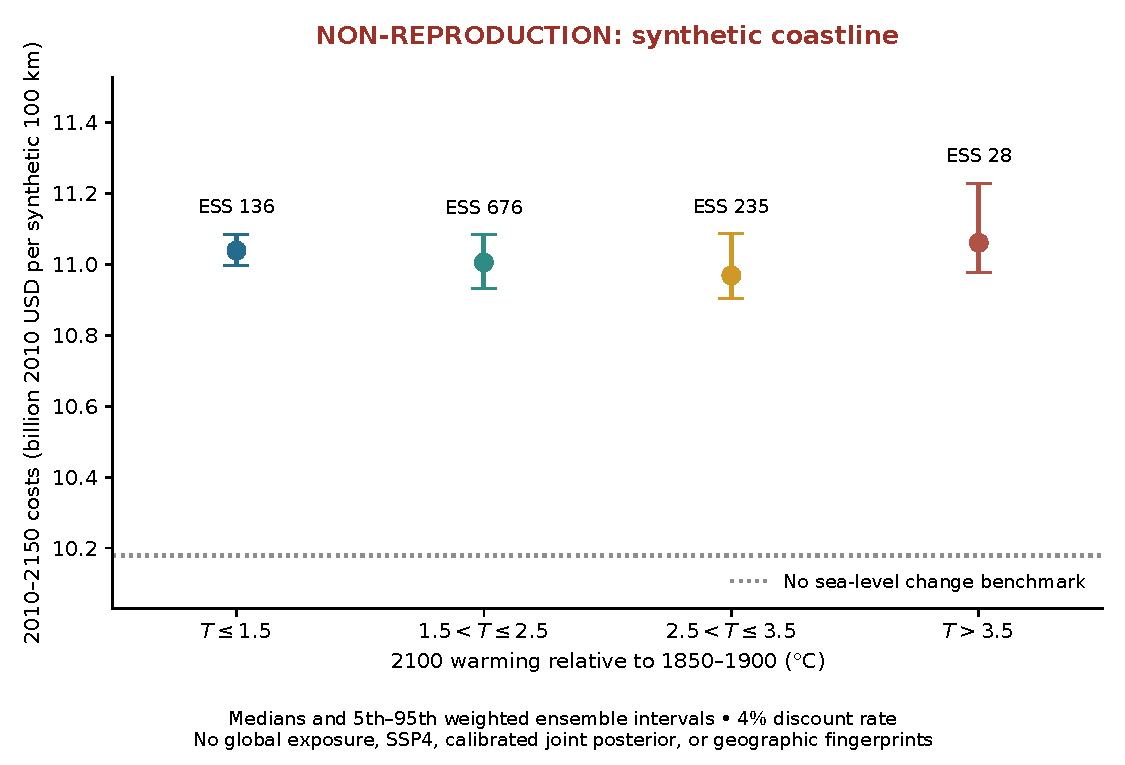
\includegraphics[width=\linewidth]{figures/figure1_nonreproduction.pdf}
\caption{Original, independently simulated \textbf{NON-REPRODUCTION} of the
conditional plotting task. Points are medians and whiskers fifth--95th
percentiles of discounted costs for a synthetic 100-km coastline. Colors
identify warming bins; labels report conditional effective sample sizes.
The dotted line retains present-day surge risk with no further sea-level
change. Units are billion 2010 dollars per synthetic coastline, not the
published trillion-dollar global quantity.}
\label{fig:one}
\end{figure}

\begin{table}[h]
\centering
% Generated by scripts/analyze.py; do not edit.
\gdef\TotalESS{1068.6}
\gdef\MaxDIC{2.2902}
\gdef\BaselineCost{10.179}
\begin{tabular}{rrrrrr}
\toprule
Bin & Draws & ESS & Probability & Median & 5th--95th \\
\midrule
1 & 200 & 135.8 & 0.121 & 11.039 & 10.998--11.085 \\
2 & 1184 & 675.6 & 0.650 & 11.005 & 10.933--11.083 \\
3 & 1368 & 234.9 & 0.214 & 10.969 & 10.904--11.086 \\
4 & 1343 & 28.1 & 0.015 & 11.061 & 10.976--11.229 \\
\bottomrule
\end{tabular}

\caption{Independent benchmark distributions. Costs are billion 2010 USD
for the 100-km test coast. Bin ordering matches Figure~\ref{fig:one}.}
\end{table}

The retained ensemble has total effective sample size \TotalESS. Its largest
surface DIC is \MaxDIC~mol/m$^3$. The no-rise counterfactual costs
\BaselineCost~billion USD2010. Initial adaptation to existing surge hazards
therefore explains much of the total cost even in cooler scenarios. The
numerical CSVs report all category quantiles, bin weights, effective tail
counts, and 400-bootstrap Monte Carlo standard errors. Prefix ensembles of
256, 512, 1024, 2048, and 4096 proposals provide a separate sampling diagnostic.
The warmest bin's low effective tail count precludes a claim of precise tail
recovery. Enlarging this ensemble would not resolve the absent global inputs.

The conditional benchmark medians are nearly flat, unlike the published
monotonic increase. Their warmest-to-coolest ratio is about 1.002. Mean
protection costs increase from 4.53 to 5.63 billion dollars between these bins,
while mean residual flood costs decrease from 5.84 to 4.77 billion dollars.
The design rule builds for the maximum water level in each foresight window,
so higher early defenses reduce near-term expected flood losses. These terms
nearly offset under 4\% discounting. This is a consequence of the synthetic
geometry, hazard, and decision rule; it is not evidence that global costs are
insensitive to warming. Without adaptation, corresponding medians increase
from 53.13 to 58.32 billion dollars. Reducing the discount rate to 2\% increases
the warmest-bin median by approximately 72\%.

\begin{table}[h]
\centering
\begin{tabular}{lrrrl}
\toprule
Warming category & Published 5th & Median & 95th & Global error\\
\midrule
$\leq1.5$ & 1.0 & 1.2 & 1.3 & undefined\\
$(1.5,2.5]$ & 1.2 & 1.5 & 2.3 & undefined\\
$(2.5,3.5]$ & 1.6 & 2.1 & unavailable & undefined\\
$>3.5$ & 2.2 & 2.6 & unavailable & undefined\\
\bottomrule
\end{tabular}
\caption{Published global costs in trillion USD2010, from manuscript prose.
Absolute and relative dollar discrepancies are undefined because this project
does not estimate the same global quantity. Unavailable values were not digitized.}
\end{table}

Published median ratios relative to the coolest bin are 1, 1.25, 1.75, and
2.167. The saved comparison table reports corresponding benchmark ratios and
their differences as descriptive shape diagnostics only. Similar ratios would
not validate synthetic exposure, and different ratios cannot isolate model
error from calibration or accounting differences.

The fixed reference model produces approximately 1.239$^\circ$C warming in
2010--2019 versus the assessed 1.06$^\circ$C, and 0.542 YJ ocean heat gain in
1971--2018 versus 0.396 YJ. These positive discrepancies are about 17\% and
37\%, respectively. Sea-level rise in 1901--2018 is approximately 0.195 m
versus 0.20 m (about $-2.5$\%). Agreement of that scalar sum does not validate
the component partition or future ice response. The 2025 CO$_2$ holdout is
reported separately in \texttt{historical\_validation.csv}; it is a short
conditional forecast, not a carbon-cycle calibration.

\begin{figure}[p]
\centering
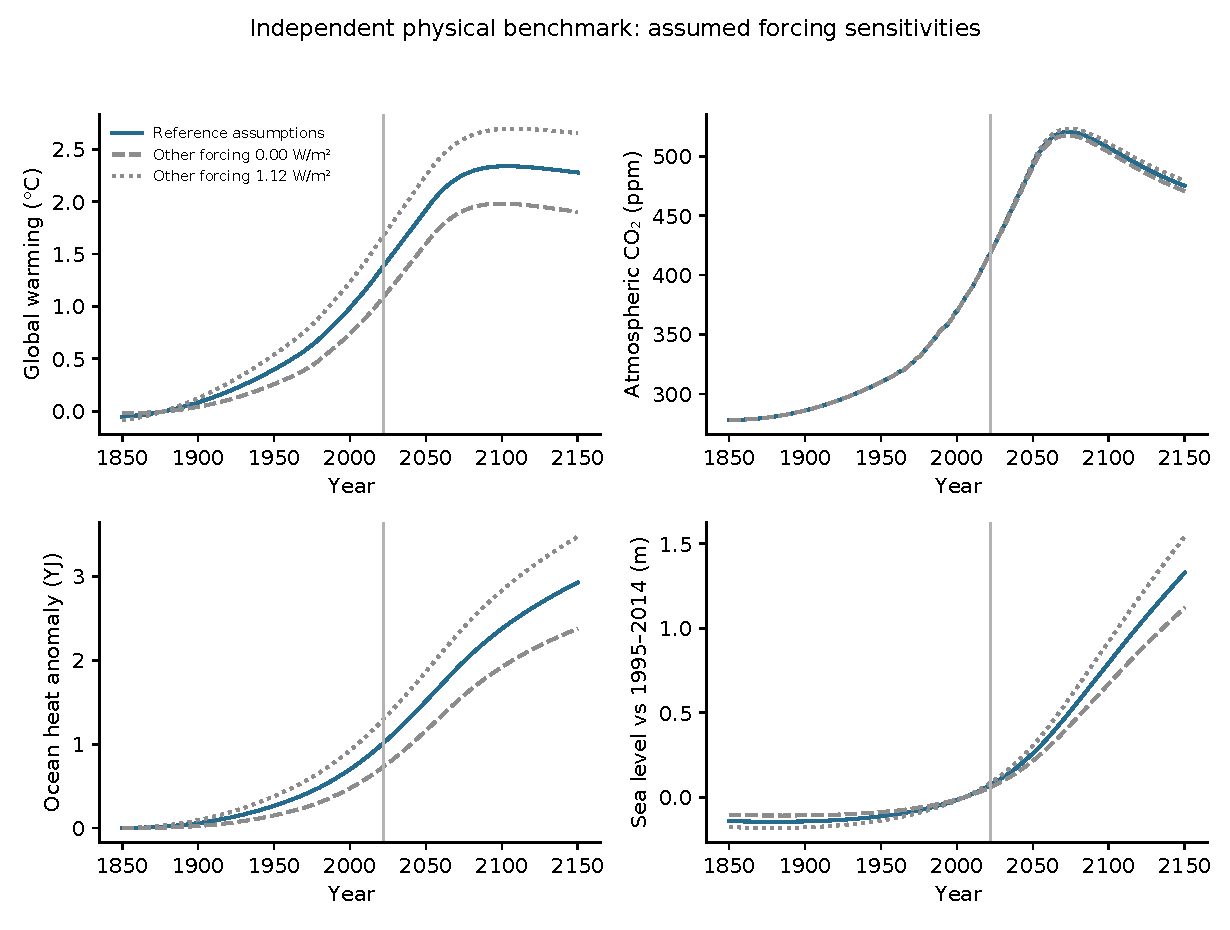
\includegraphics[width=\linewidth]{figures/physical_diagnostics.pdf}
\caption{Reference physical trajectories and sensitivity to assumed other
forcing of 0, 0.56, and 1.12 W/m$^2$ after 2019. All curves are independent
model output. Temperature uses 1850--1900 and sea level 1995--2014 references;
heat is the anomaly from the 1850 initial state. The vertical line marks the
2022 switch from prescribed CO$_2$ to emissions forcing. Historical prescribed
CO$_2$ agreement is a boundary condition, not a validation result.}
\end{figure}

\section{Verification, limitations, and next steps}
The verification executable checks zero forcing, doubled-CO$_2$ equilibrium,
global heat conservation, terrestrial equilibrium, carbon pulse conservation,
the reconstructed ocean impulse response, Antarctic reference radius and
volume, its volume derivative and mass balance, exact reference-period
normalizations, prescribed CO$_2$, cost accounting, and analytic flood
integration against numerical quadrature. The reference Antarctic radius
differs from 1.864 million metres by about 0.019\%; volume differs from
$24.78\times10^{15}$ m$^3$ by about 0.003\%. Carbon budget residuals are of
order $10^{-12}$ Gt C per step, and heat residuals about $10^{-15}$ YJ per step.

Refinement from a half-year to an eighth-year step at 80 ocean cells changes
2100 warming by about $10^{-5}$~$^\circ$C and sea level by $2.3\times10^{-5}$~m.
At half-year steps, 40 versus 160 cells changes warming by about 0.0008$^\circ$C
and sea level by 0.0005 m. Cost changes are below 0.01\%. Climate and carbon
convergence is approximately second order after correcting the historical
boundary. The ice model's activation conditions and adaptation choices are
nonsmooth, so a single formal convergence order is not claimed for all outputs.
The refinement tolerances are 0.02$^\circ$C, 0.02 m, and 1\% cost; they test
numerical resolution rather than scientific accuracy.

One initial 4096-proposal run failed the all-members carbonate-domain check.
The corrected analysis explicitly records exclusions and their pre-filter
weight; it does not conceal the failed check. The primary experiments use one
CPU, with no large spatial data products. Source and compact numerical results
are retained. The build compiles the C++ model, runs tests and experiments,
generates original plots, and compiles this report without network access.

Exact Figure 1 reproduction remains blocked by missing joint calibration and
emission probabilities, the unresolved supplement, incomplete forcing and
rapid-Antarctic configuration, absent fingerprint and land-motion grids, and
unrecovered coastal exposure, hazard, SSP4, and economic parameters. The GTSR
archive was identified but could not be retrieved in this environment.
These are scientific-input and access limitations, not numerical instabilities.
They affect the probability measure and even the definition of the economic
quantity, so they cannot be represented by enlarging Monte Carlo error bars.

The existing Git metadata is read-only. Checkpoints were therefore stored in
a separate writable Git database inside the project. GitHub API requests fail;
the CLI also reports an invalid token for its locally named account. Remote
identity, repository existence, and public visibility could not be verified.
No public repository or successful push is claimed. Source checkpoints and a
portable bundle preserve the work for later publication.

The next scientific step is to obtain the missing written configuration and
independent geographic inputs with verified licenses, then calibrate the
reconstructed forward system against the specified time series. Only after
matching local sea-level mapping, exposure, SSP4, and accounting conventions
would a global dollar comparison be interpretable. This benchmark establishes
a tested computational starting point and identifies the boundaries of what
its present outputs can support.

\begin{thebibliography}{99}
\bibitem{wong2025} Wong et al. (2025). Coastal adaptation and damage costs at
different global warming thresholds. \emph{npj Natural Hazards} 2, 35.
\href{https://doi.org/10.1038/s44304-025-00089-0}{doi:10.1038/s44304-025-00089-0}.
\bibitem{urban} Urban and Keller (2010). Probabilistic hindcasts and projections
of the coupled climate, carbon cycle and Atlantic meridional overturning
circulation system. \emph{Tellus A}.
\href{https://doi.org/10.1111/j.1600-0870.2010.00471.x}{doi:10.1111/j.1600-0870.2010.00471.x}.
\bibitem{kriegler} Kriegler (2005). \emph{Imprecise probability analysis for
integrated assessment of climate change}. Doctoral dissertation, University of Potsdam.
\href{https://www.pik-potsdam.de/members/edenh/theses/PhDKriegler.pdf}{Written source}.
\bibitem{ricciuto} Ricciuto, Davis, and Keller (2008). A Bayesian calibration
of a simple carbon cycle model. \emph{Global Biogeochemical Cycles} 22, GB2030.
\href{https://doi.org/10.1029/2006GB002908}{doi:10.1029/2006GB002908}.
\bibitem{tanaka} Tanaka (2007). \emph{Inverse estimation for the simple Earth
system model ACC2 and its applications}. Doctoral dissertation. Eqs. 2.1.11--12.
\bibitem{yi} Yi et al. (2001). The effects of buffer and temperature feedback
on the oceanic uptake of CO$_2$. \emph{Geophysical Research Letters}.
\href{https://doi.org/10.1029/2000GL011569}{doi:10.1029/2000GL011569}.
\bibitem{dcess} Fern\'andez Villanueva and Shaffer (2025). DCESS II.
\emph{Geoscientific Model Development} 18, 2161--2192.
\href{https://doi.org/10.5194/gmd-18-2161-2025}{doi:10.5194/gmd-18-2161-2025}.
\bibitem{brick} Wong et al. (2017). BRICK v0.2, a simple, accessible, and
transparent model framework for climate and regional sea-level projections.
\emph{Geoscientific Model Development} 10, 2741--2760.
\href{https://doi.org/10.5194/gmd-10-2741-2017}{doi:10.5194/gmd-10-2741-2017}.
\bibitem{shaffer} Shaffer (2014). Formulation, calibration and validation of
the DAIS model (version 1). \emph{Geoscientific Model Development} 7, 1803--1818.
\href{https://doi.org/10.5194/gmd-7-1803-2014}{doi:10.5194/gmd-7-1803-2014}.
\bibitem{diam} Diaz (2016). Estimating global damages from sea level rise with
the Coastal Impact and Adaptation Model (CIAM). \emph{Climatic Change}.
\href{https://doi.org/10.1007/s10584-016-1675-4}{doi:10.1007/s10584-016-1675-4}.
\bibitem{ciam} Wong et al. (2022). Sea level and socioeconomic uncertainty
drives high-end coastal adaptation costs. \emph{Earth's Future}.
\href{https://doi.org/10.1029/2022EF003061}{doi:10.1029/2022EF003061}.
\bibitem{noaa} NOAA Global Monitoring Laboratory (2026). Trends in atmospheric
carbon dioxide, annual mean Mauna Loa record. Snapshot dated 9 October 2026.
\href{https://gml.noaa.gov/webdata/ccgg/trends/co2/co2_annmean_mlo.txt}{Data source}.
\bibitem{ipcc} IPCC (2021). Climate Change 2021: The Physical Science Basis.
Working Group I, Summary for Policymakers and Chapters 7 and 9.
\href{https://www.ipcc.ch/report/ar6/wg1/}{Assessment source}.
\end{thebibliography}
\end{document}
